\documentclass[xetex,mathserif,serif]{beamer}
\usetheme{Madrid}
\title{TRANSFER LEARNING FOR ONE-CLASS RECOMMENDATION BASED ON MATRIX FACTORIZATION}
\author{XIE Ruiming}
\date{2015.02.12}
\begin{document}
\frame{\titlepage}
\begin{frame}
  \frametitle{Outline}
  \tableofcontents
\end{frame}
\AtBeginSection[]
{
  \begin{frame}
    \frametitle{Outline}
    \tableofcontents[currentsection]
  \end{frame}
}
\begin{section}{Background}
  \begin{frame}{Traditional recommender system}
    \begin{center}
      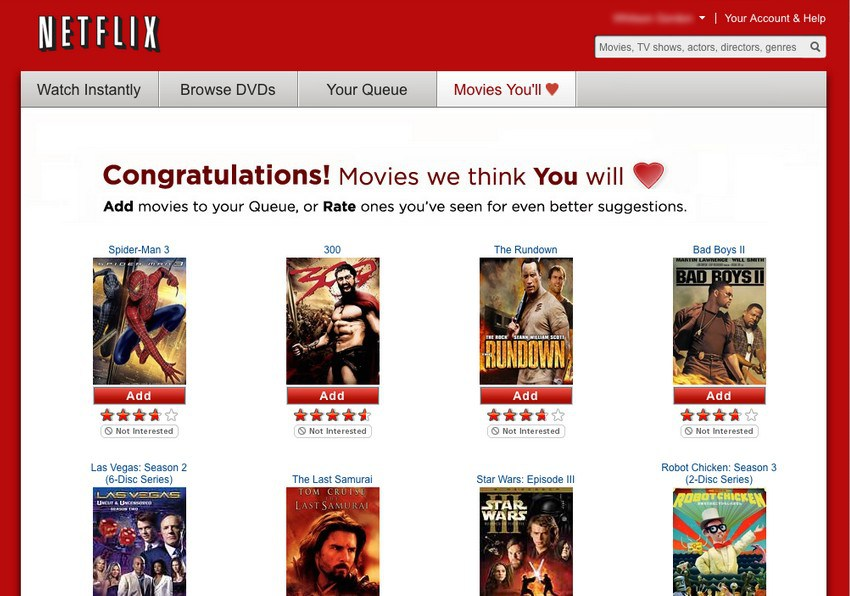
\includegraphics[width=0.7\textwidth]{fig/netflix.jpg}
    \end{center}
    The data have multiple values(ratings from 1 to 5).
  \end{frame}
  \begin{frame}{One-class recommender system}
    \begin{center}
      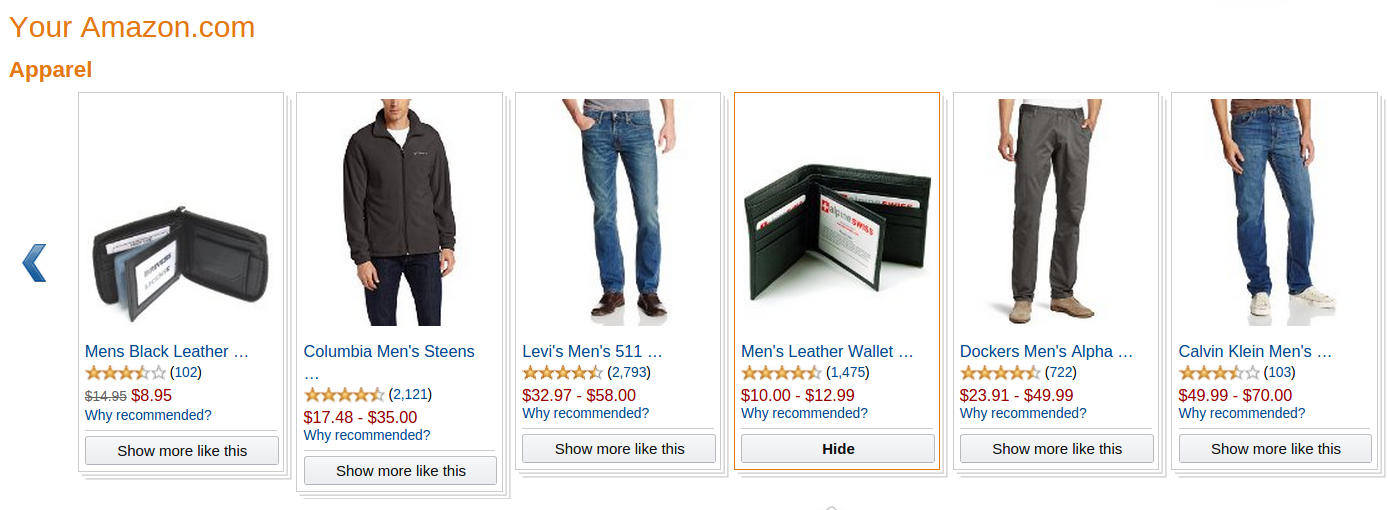
\includegraphics[width=0.9\textwidth]{fig/amazon.png}
    \end{center}
    The data usually are binary. No ratings are available.
  \end{frame}

  \begin{frame}{Matrix factorization \& Transfer Learning}
    \begin{block}{Matrix factorization}
      Matrix factorization models map both users and items to a
      joint latent factor space of dimensionality f, such that user-item interactions are modeled as inner products in that space.

      \alert{Matrix tri-factoriztion} factorizes a matrix $M$ into three parts : $M = USV^T$. Where $U,V$ stand for user/item clusters and $S$ stands for cluster relationships.
    \end{block}

    \begin{block}{Transfer Learning}
      As a way to transfer knowledge from different domains, transfer learning can be applied in recommender systems to leverage data in different system with shared users.

      There exists some research that use transfer learning to tackle CF problems.
    \end{block}
  \end{frame}

  \begin{frame}
    \begin{center}
      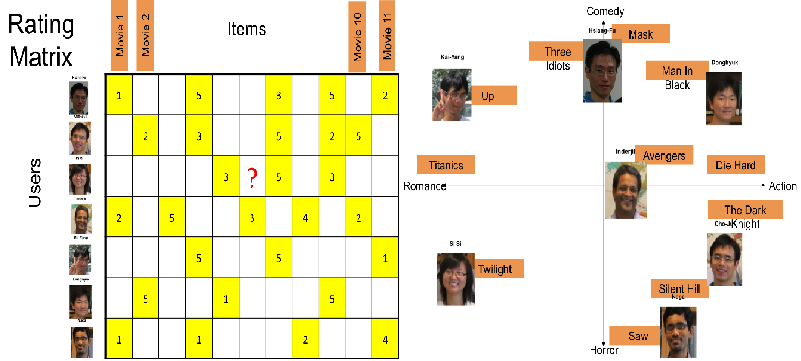
\includegraphics[width=\textwidth]{fig/pmf.png}
    \end{center}
  \end{frame}

\end{section}

\begin{section}{Motivation}
  \begin{frame}
    \frametitle{Motivation}
    \begin{itemize}
    \item Users often have different kinds of actions in one website. We can treat different actions as different domains and adopt transfer learning methods.
    \item The actions are mostly binary.
    \item Current methods can't solve transfer learning in one-class recommendation.
    \end{itemize}
  \end{frame}
\end{section}

\begin{section}{Transfer Learning in One Class CF for Shopping Prediction}
  \begin{frame}
    \frametitle{TRIMF}
    \begin{block}{Problem background}
      \begin{itemize}
      \item
        \par{In an online shopping site, there are two main actions - click and purchase. Both can form a matrix which consists of binary data. And the primary goal for the site is to increase \alert{conversion rate}.}
      \item
        \par{The matrices are sparse, but add them together into one matrix is too simple to success. So we need to consider a transfer learning method to leverage data better.}
      \end{itemize}
    \end{block}
  \end{frame}
  \begin{frame}
    \frametitle{Problem Definition}
    \begin{itemize}
    \item Input: click matrix $X_c^{m_c*n_c}$, deal matrix $X_d^{m_d*n_d}$

      $m_c,m_d$ are the number of users in each matrix while $n_c,n_d$ denote the number of items.
    \item Output: prediction matrices $P_c^{m_c*n_c}, P_d^{m_d*n_d}$.
    \end{itemize}
  \end{frame}
  \begin{frame}
    \frametitle{Weighting scheme}
    Former one-class CF methods aim at giving entries different weights. Thus different confidence levels can be set. TRIMF combines two weight schemes together.
    \begin{itemize}
    \item Positive entries: $W_{ij} = 1 + log(n)$
      \begin{itemize}
      \item Higher frequency can mean that we are more confident about the entry.
      \end{itemize}
    \item Negative(Unknown) entries: $W_{ij} = log(\sum_j X_{ij})$
      \begin{itemize}
      \item If a user has more positive examples, it is more
        likely that the user does not like the missing items.
      \end{itemize}
    \end{itemize}
  \end{frame}
  \begin{frame}
    \frametitle{Clustering effects in shopping site}
    \begin{table}[h]
      \begin{center}
        \begin{tabular}{| c | c |}
          \hline
          Top click items & Top purchase items \\
          \hline
          Iphone 5s & Tissue\\
          Xiaomi 3 & Laundry soap powder\\
          Thinkpad & Xiaomi 3\\
          CPU & Snacks\\
          Hard disk & Battery\\
          Router & Iphone 5s\\
          Earphone & Mouse\\
          \hline
        \end{tabular}
        \caption{Top 10 click items and purchase items in Yixun.}
      \end{center}
      % \end{Large}
    \end{table}
    There are some categories which users tend to buy after click. Also users have different shopping habits, some like window-shopping and some like to buy right after clicking.
  \end{frame}
  \begin{frame}
    \frametitle{Transfer Learning in TRIMF}
    Traditional transfer methods in CF only share a certain part of matrices through \alert{matrix tri-factorization}.

    TRIMF shares user-latent factors and rating patterns, while designing a cluster-level mapping function.
  \end{frame}
  \begin{frame}
    \frametitle{TRIMF}
    \begin{block}
      {Objective function}
      {$$min_{F,G,S,U,V} W_c\odot ||X_c - (F;F_c)S(G;G_c)'||_2$$ $$+ W_d\odot ||X_d - (F;F_d)(USV)(G;G_d)'||_2 $$}
    \end{block}
    \begin{itemize}
    \item $W_c,W_d$ are the weights for $X_C, X_d$.
    \item $F, G$ are the soft clustering result matrices for overlapped users(items), they are forced to be the same. $F_c,F_d,G_c,G_d$ are matrices for unique users(items).
    \item $U,V$ are two diagonal matrices, $U_{ii}$ scales every $S_{i*}$ to $U_{ii}S_{i*}$, and models the users' cluster-level transformation from click to deal. While $V_{jj}$ scales every $S_{*j}$ to $S_{*j}V_{jj}$, it models the items' cluster-level transformation from click to deal.
    \end{itemize}
  \end{frame}
  \begin{frame}
    \frametitle{TRIMF}
    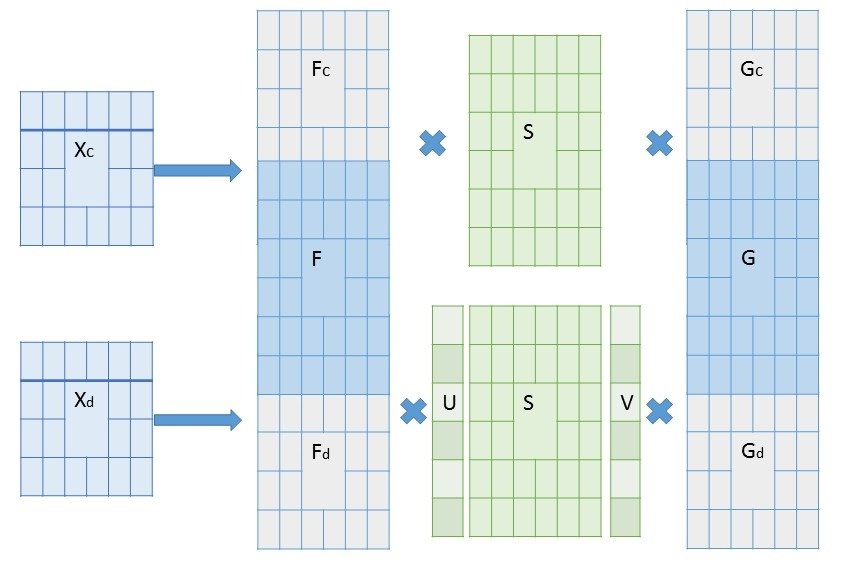
\includegraphics[width=\textwidth]{fig/trimf.jpg}  
  \end{frame}

\end{section}

\begin{section}{Clustering-based Matrix Factorization for Online Shopping Prediction}
  \begin{frame}
    \frametitle{Limitation of TRIMF}
    \par{ When data are coming from multiple sources (e.g. click, pageview and add cart), TRIMF treats every source equally and puts each of them into one matrix which is very sparse. More actions will produce more matrices, increasing complexity.}
    \par{What is more, in reality the data is much sparser than datasets in experiment. We cannot guarantee achieving equal performance.}
  \end{frame}
  \begin{frame}
    \frametitle{CBMF}
    \begin{columns}
      \begin{column}{0.6\textwidth}
        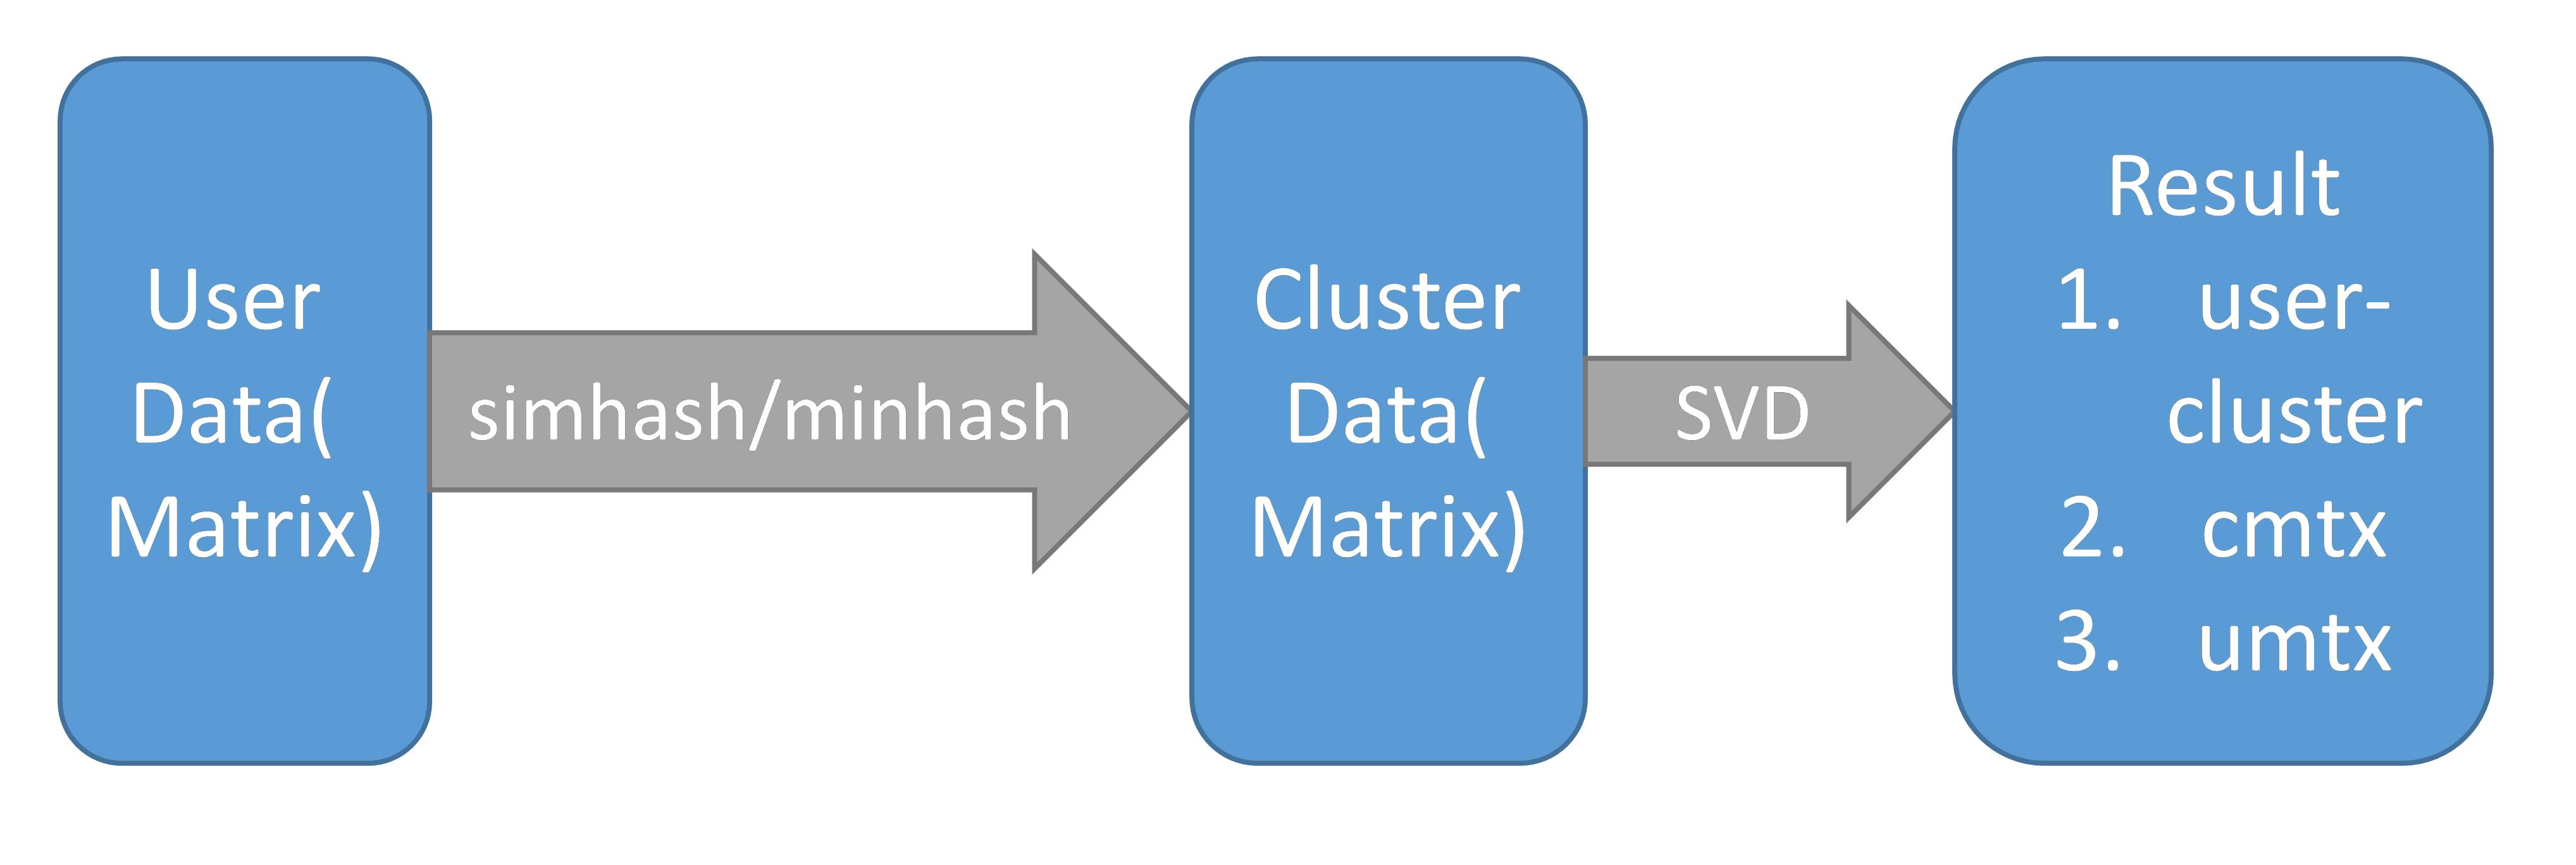
\includegraphics[width=\textwidth]{fig/d.jpg}
      \end{column}
      \begin{column}{0.35\textwidth}
        we have developed a matrix factorization framework based on a clustering and scoring scheme(CBMF). And apply it in an online shopping site(Tencent).
      \end{column}
    \end{columns}
  \end{frame}
  \begin{frame}
    \frametitle{Clustering method in CBMF}
    In Tencent, we have 800,000,000 users in total, and their feature vectors dimensions can be as large as 1,000,000. Our method first convert sparse vectors into dense vectors(Simhash) then perform one-phase clustering(Minhash).
    \begin{block}{Simhash}
      Simhash is a kind of locality sensitive hashing(LSH) where similiar items are hashed to similiar hash values. We can use \alert{hamming distance} between two hase values to compare their similarity.
    \end{block}

  \end{frame}
  \begin{frame}
    \frametitle{Clustering method in CBMF}
    \begin{block}
      {Jaccard similarity}
      The Jaccard similarity coefficient is a commonly used indicator of the similarity between two sets:$$J(A, B) = \frac{A \cup B}{A \cap B}$$              
    \end{block}
    \begin{block}
      {Minhash}
      Let $h$ be a hash function, and for any set $S$ define $h_{min}(S)$ to be the minimal member of $S$ with respect to $h$. The probability that $h_{min}(A) = h_{min}(B)$ is true is equal to the similarity $J(A,B)$.
    \end{block}
    We can produce multiple $h^i_{min}A$ for each set then concatenate them together as our hash-key. The probability that two sets $A,B$ will agree the concatenated hash-key is equal to $J(A,B)^p$.
  \end{frame}
  \begin{frame}
    \frametitle{Simhash \& Minhash using MapReduce}
    \begin{itemize}
    \item Map(input:user vector $u_i$):
      \begin{itemize}
      \item calculate Simhash of $u_i$, $s(u_i)$
      \item calculate Minhash of $s(u_i)$ for $p$ times, concatenate them together.
      \item output $(minhash_i, u_i)$, $minhash_i$ is the cluster id of $u_i$
      \end{itemize}
    \item Reduce:
      \begin{itemize}
      \item for one $minhash_i$, add all vectors that belong to $minhash_i$ together then normalize it. We can generate a cluster-vector $c_i$.
      \item output $(minhash_i, c_i)$.
      \end{itemize}
    \end{itemize}
  \end{frame}
  \begin{frame}
    \frametitle{Feature scoring in CBMF}
    \begin{itemize}
    \item     A user can have many actions, including click, purchase and pageview. CBMF integrate these actions into one matrix. For a specific action to an item, the score given should depend on how much impact the action has. 

    \item  For example, the conversion rate for item iPhone 6 is $CVR(iphone6_{all})$. The conversion rate for iPhone 6 in people who had clicked it is $CVR(iphone6_{click})$. Then their log ratio $log(\frac{CVR(iphone6_{click})}{CVR(iphone6_{all})})$ becomes our score for click. 

    \item We add a weighted sum for all actions as our final score.
    \end{itemize}
  \end{frame}
  \begin{frame}
    \frametitle{Matrix factorization in CBMF}
    \begin{itemize}
    \item Once the matrices are generated, we use Singular Value Decomposition(SVD) from mahout to produce our results.
    \item For expericeced users we provide a mixed result(direct and clustering), for new users we provide results from his cluster.
    \end{itemize}
    
  \end{frame}
\end{section}

\begin{section}{Experiments}
  \begin{frame}
    \frametitle{Offline experiments}
    \begin{block}
      {Datasets}
      \begin{itemize}
      \item Yixun: A dataset from Yixun, a large online retailer for electronic products, that has been sampled from log data from two weeks.
      \item Tmall: A similar but smaller anonymized dataset from a shopping portal containing user interactions of different types.
      \end{itemize}
      \begin{table}
        \begin{center}
          \begin{tabular}{c c c}
            \hline
            Datasets & Yixun & Tmall\\
            \hline
            users(click) & 16,240 & 884\\
            % \hline
            items(click) & 1,932 & 9,531\\
            % \hline
            sparsity(click) & 0.006 & 0.021\\
            % \hline
            \hline
            users(purchase) & 2,520& 884\\
            % \hline
            item(purchase) & 1,791& 4,312\\
            % \hline
            sparsity(purchase) & 0.0003 & 0.001\\
            \hline
          \end{tabular}
        \end{center}
        \caption{Dataset characteristics.}
        \label{dataset}


      \end{table}
    \end{block}
  \end{frame}
  \begin{frame}
    \frametitle{Metric}
    We use $prec@5$ and $prec@10$ as our evaluation metrics. Precision is the fraction of clicked items that are shown to the user. $$Precision = \frac{\|click\|}{\|Impression\|}$$

    \par{Precision takes all retrieved documents into account, but it can also be evaluated at a given cut-off rank, considering only the topmost results returned by the system. This measure is called \textbf{precision at n} or \textbf{$prec@n$}.}
  \end{frame}
  \begin{frame}
    \frametitle{Baseline methods}
    \begin{itemize}
    \item non-transfer:
      For all non-transfer methods, we use three combinations of matrices as our training matrix:{deal, click, deal+click}, and report their \alert{best} performance.
      \begin{itemize}
      \item \textbf{Most Popular}: selects top-n items globally, and provides the same recommendation results for every user.
      \item \textbf{Singular Value Decomposition(SVD)}: a typical method used in recommender system.
      \item \textbf{Non-negative Matrix Factorization(NMF)}.
      \item \textbf{Probabilistic Matrix Factorization(PMF)}: a recently proposed method for missing value prediction.
      \item \textbf{BPRMF}: BPR is a generic optimization criterion for personalized ranking. Unlike traditional methods whose objective function is point-wise, BPR is a pair-wise object function. BPRMF implements BPR using matrix factorization.
      \item \textbf{WRMF}: One-class collaborative filtering(WRMF) is a weighted low rank approximation method optimized for an implicit dataset. 
      \end{itemize}
    \end{itemize}
  \end{frame}
  \begin{frame}
    \frametitle{Baseline methods}
    \begin{itemize}
    \item transfer methods:
      \begin{itemize}
      \item \textbf{Collective Matrix Factorization(CMF)}: is proposed for jointly factorizing two matrices. CMF has been proven to be an effective cross-domain recommendation approach. 
      \item \textbf{TCF}: is a transfer learning method used to predict missing ratings via heterogeneous feedback.
      \end{itemize}
    \end{itemize}
  \end{frame}
  \begin{frame}
    \frametitle{Offline experiment results}
    \begin{table}


      \begin{center}
        \begin{tabular}{|c|c|c|}
          \hline
          Method&Prec@5&Prec@10\\
          \hline
          Most Popular&0.0323&0.0289\\
          \hline
          SVD&0.0438&0.0367\\
          \hline
          NMF&0.0403&0.0324\\
          \hline
          PMF&0.0435&0.0372\\
          \hline
          BPRMF&0.0444&0.0364\\
          \hline
          WRMF&0.049&0.0403\\
          \hline
          CMF&0.0436&0.0350\\
          \hline
          TCF&0.0453&0.0369\\
          \hline
          TRIMF&\textbf{\color{red}0.0525}&\textbf{\color{red}0.0410}\\
          \hline
          CBMF&\textbf{0.512}&\textbf{0.403}\\
          \hline
        \end{tabular}
      \end{center}
      \caption{Performance comparision on Yixun users who have deal data.}
      \label{shortdeal}

    \end{table}
  \end{frame}
  \begin{frame}
    \frametitle{Offline experiment results}
    \begin{table}

      \centering


      \begin{tabular}{|c|c|c|}
        \hline
        Method&Prec@5&Prec@10\\
        \hline
        Most Popular&0.0090&0.0085\\
        \hline
        SVD&0.0123&0.00113\\
        \hline
        NMF&0.0091&0.0089\\
        \hline
        PMF&0.0121&0.0112\\
        \hline
        BPRMF&0.0142&0.0130\\
        \hline
        WRMF&0.0174&0.0144\\
        \hline
        CMF&0.0176&0.0139\\
        \hline
        TCF&0.0158&0.0127\\
        \hline
        TRIMF&\textbf{\color{red}0.0189}&\textbf{\color{red}0.0153}\\
        \hline
        TRIMF(without remap)&0.0175&0.0146\\
        \hline
        CBMF&\textbf{0.0181}&\textbf{0.0144}\\
        \hline
      \end{tabular}
      \caption{Performance comparision on Yixun users who have click data.}
      
    \end{table}
  \end{frame}
  \begin{frame}
    \frametitle{Offline experiment results}
    \begin{table}
      \centering
      \begin{tabular}{|c|c|c|}
        \hline
        Method&Prec@5&Prec@10\\
        \hline
        Most Popular&0.00508&0.00405\\
        \hline
        SVD&0.00453&0.00413\\
        \hline
        NMF&0.00401&0.00389\\
        \hline
        PMF&0.00421&0.00312\\
        \hline
        BPRMF&0.00542&0.00430\\
        \hline
        WRMF&0.00485&0.00345\\
        \hline
        CMF&0.00512&0.00432\\
        \hline
        TCF&0.00534&0.00502\\
        \hline
        TRIMF&\textbf{\color{red}0.00720}&\textbf{\color{red}0.00606}\\
        \hline
        CBMF&\textbf{0.00612}&\textbf{0.00503}\\
        \hline
      \end{tabular}
      \caption{Performance comparision on Tmall users.}
    \end{table}
  \end{frame}
  \begin{frame}
    \frametitle{Offline experiment analysis}
    \begin{block}{The effects of cluster-level transformation} 
      \begin{itemize}
      \item 
        In our assumption, $U,V$ are two mapping matrices that describe the difference in user clusters and item categories. To see whether $U,V$ really reflect the phenomenon, we manually check entries in $U,V$ with high and low values. We found that high values in $V$ reflect item clusters that people tends to buy after clicking, e.g. toothbrush, snacks. While low values of $V$ more reflects items that are popular but people may not buy immediately, e.g. cell phones and laptops.
      \item If we map $UV$ back to the click matrix. Thus the learned cluster-pattern $S$ is transformed from the click pattern to the purchase pattern.
      \end{itemize}
    \end{block}
  \end{frame}
  \begin{frame}
    \frametitle{Offline experiment analysis}
    \begin{block}
      {The effects of latent vector sharing}
      \begin{itemize}
      \item In TRIMF, for the same user the latent vectors are unique. 
      \item To see that sharing $F,G$ really works, we randomly select another 6000 users and 1500 items from Yixun, make two new matrices $X'_c, X'_d$ to perform another test.
        \begin{itemize}
        \item share$FG$ : TRIMF
        \item not share : we update $F_c, G_c, F_d, G_d$ separately, pretending there is no overlapping users or items.
        \item random share : we randomly choose 3000 users and 800 items, marking them as overlapping,
        \end{itemize}
      \end{itemize}
    \end{block}
  \end{frame}
  \begin{frame}
    \frametitle{Offline experiment analysis}
    \begin{table}
      \begin{center}
        \begin{tabular}{|c|c|c|}
          \hline
          Method&Prec@5&Prec@10\\
          \hline
          share$FG$&\textbf{\color{red}0.0436}&\textbf{\color{red}0.0350}\\
          \hline
          not share&0.0335&0.0306\\
          \hline
          random share&0.0344&0.0299\\
          \hline
        \end{tabular}
      \end{center}
      \caption{The effect of sharing.}
      \label{sharing}
    \end{table}
  \end{frame}
  \begin{frame}
    \frametitle{Scalability}
We select the Yixun dataset. We implement TRIMF and CBMF using Python 2.7 with Numpy and Scipy, and run them using a laptop with Intel Core i5-4200 with 4 cores at 2.4GHz and 12GB memory.

For each method, the update algorithm stops while training loss is less than $n$. 

\begin{itemize}

\item we set different threshold for $n$, and test the convergence speed for each method. 
\item we reduce the size of click matrix, and test the training speed regarding to dataset size. 
\item we set different number of parameters(latent dimension k) for each method, and test the training speed with regard to parameter size. 
\end{itemize}
  \end{frame}

  \begin{frame}
    \frametitle{Scalability}
    \begin{figure}
    \begin{center}
    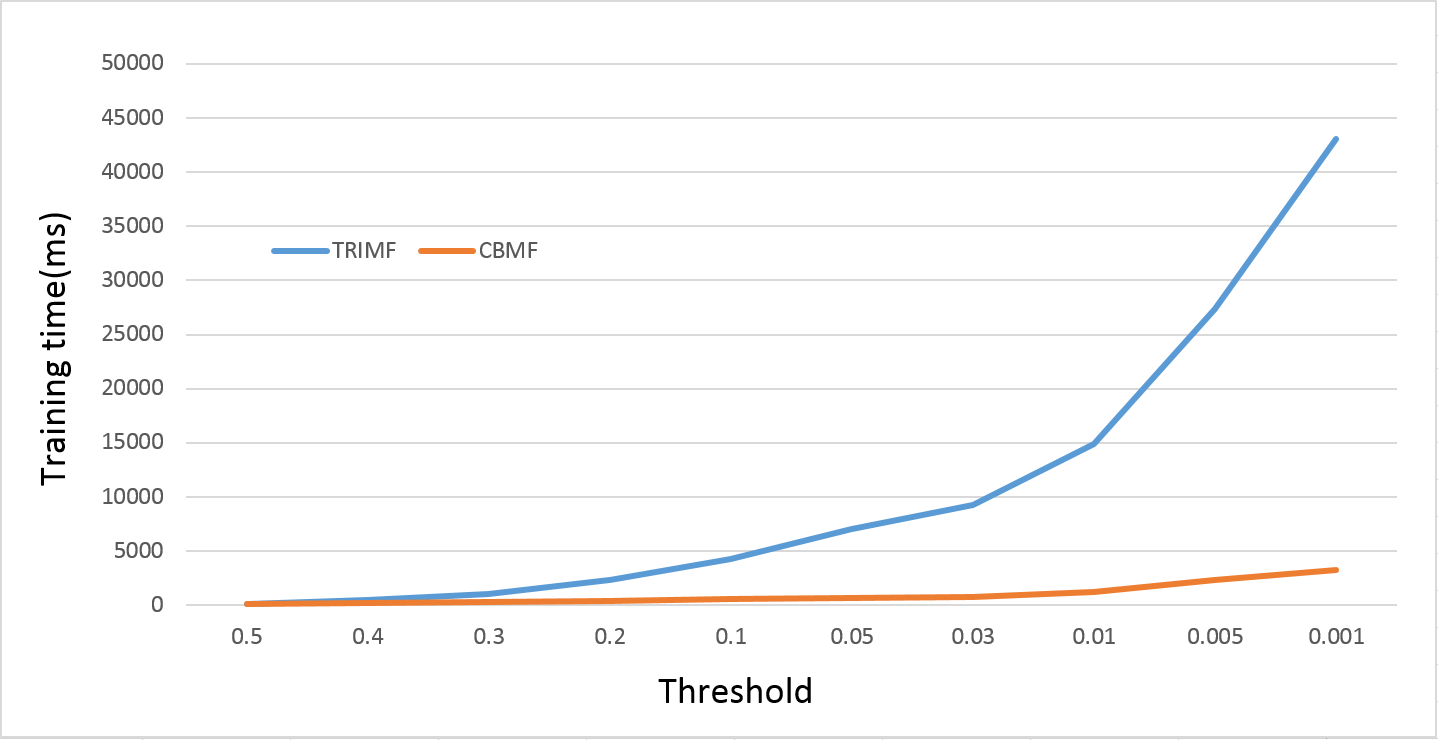
\includegraphics[width=0.9\textwidth]{fig/cbmf1.png} 
    \caption{Convergence speed with regard to threshold.}

  \end{center}
\end{figure}
\end{frame}

  \begin{frame}
    \frametitle{Scalability}
    \begin{figure}
    \begin{center}
    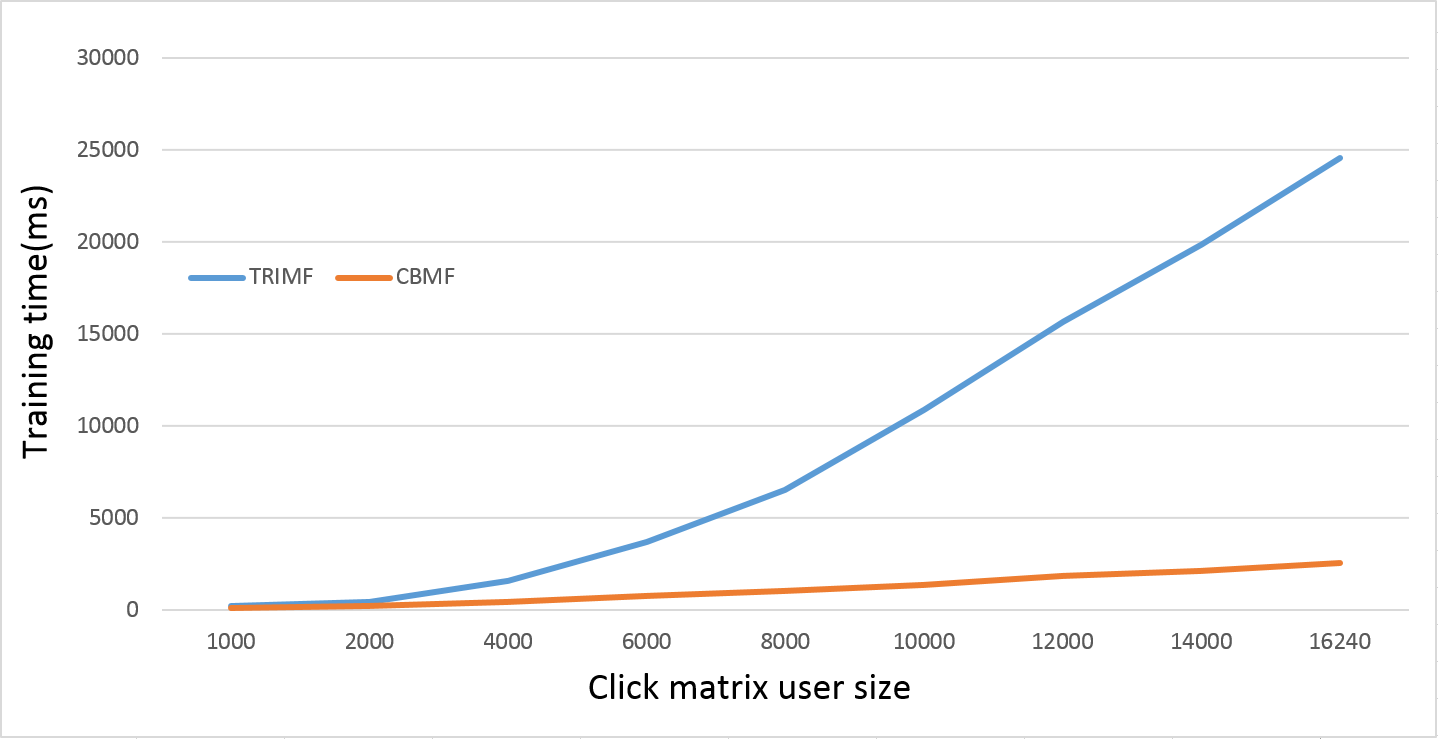
\includegraphics[width=0.9\textwidth]{fig/cbmf2.png} 
    \caption{Convergence speed with regard to data size.}

  \end{center}
\end{figure}
\end{frame}


  \begin{frame}
    \frametitle{Scalability}
        \begin{figure}
    \begin{center}
    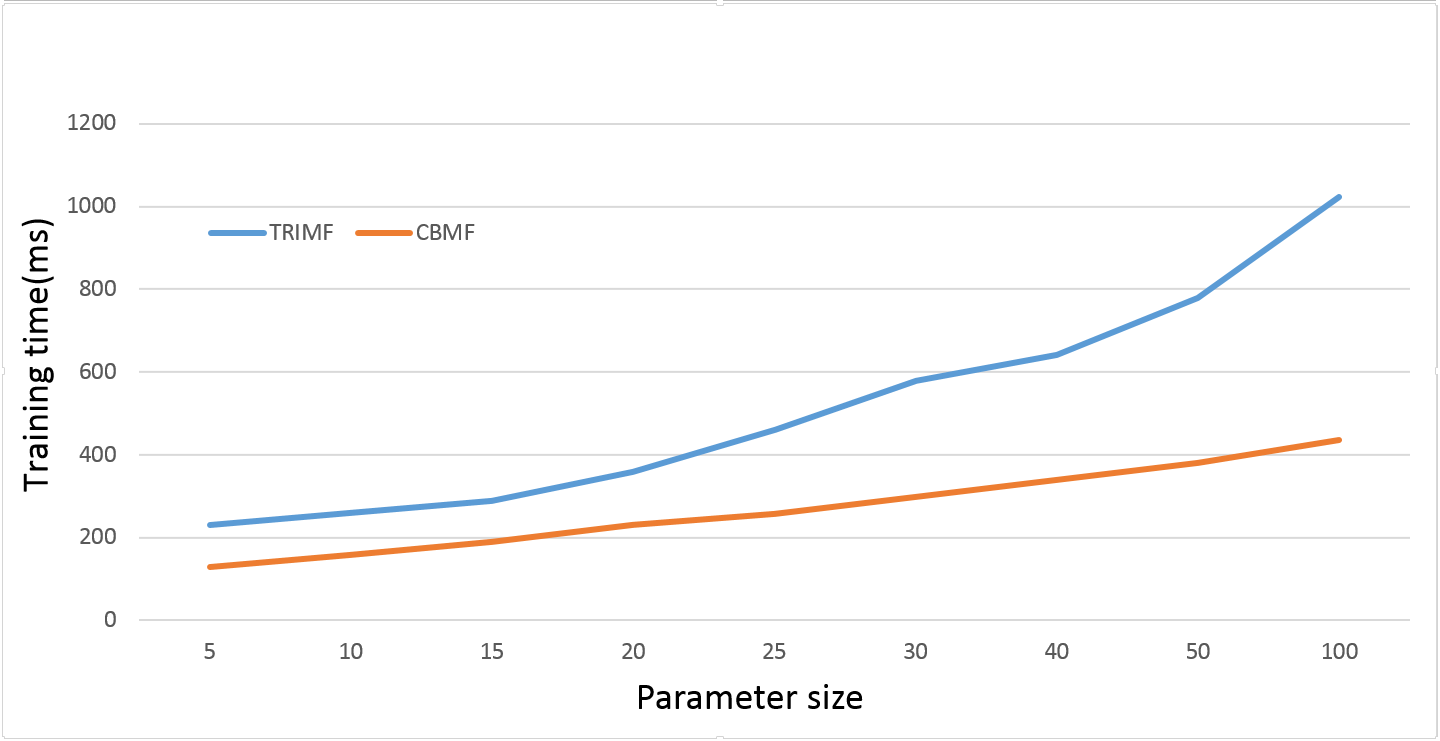
\includegraphics[width=0.9\textwidth]{fig/cbmfsize.png} 
    \caption{Convergence speed with regard to parameter size.}

  \end{center}
\end{figure} 
\end{frame}

\begin{frame}
  \frametitle{Online experiments}

\end{frame}
\begin{frame}
  \frametitle{Online experiments metrics}
An impression is a measure of the number of times an advertisement is seen. 
\begin{itemize}
\item  click-through-rate(CTR). The click-through rate is the number of times a click is made on the advertisement divided by the total impressions (the number of times an advertisement was served). $$CTR = \frac{Clicks}{Impressions} * 100\%$$
\item  order amount per impression(OAPI). $$OAPI = \frac{Order \,\,Prices}{Impressions}$$
\item  pay amount per impression(PAPI). $$PAPI = \frac{Paid \,\,Money}{Impressions}$$
\end{itemize}
\end{frame}
\begin{frame}
  \frametitle{Online experiment baselines}
\begin{itemize}

\item \textbf{Co-clustering CF} (4313) is a scalable collaborative filtering framework based on co-clustering. Previous work showed that this method had a fast training time while providing decent accuracy.
\item \textbf{Factorization Machine} (4314) is a generic approach that allows to mimic most factorization models by feature engineering. It provides high accuracy in several important prediction problems including recommender systems.
\item \textbf{Item-based CF} (4315) is a typical recommending method proposed by Amazon. Cosine distance is used in calculating item similarities.
\item \textbf{Efficient top-n recommendation} (cpsf) is a recommendation pipeline, which is the winner of the Million Songs Dataset (MSD) challenge.
\item \textbf{CBMF}(4312): Our method.

\end{itemize} 
\end{frame}
\begin{frame}
  \frametitle{Online experiment results}
\begin{figure}
\begin{center}
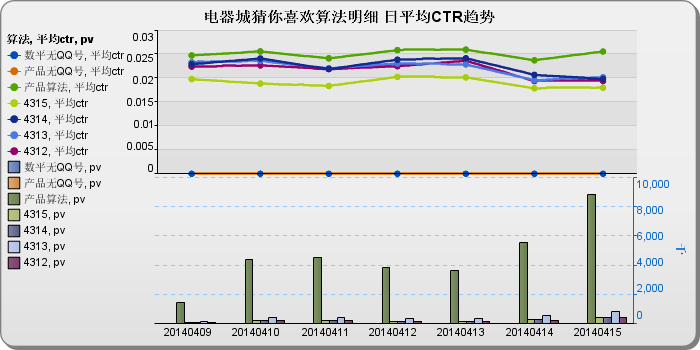
\includegraphics[width=0.8\textwidth]{fig/ctr0415.png}
\caption{ CTR of online algorithms from 0409 to 0415.}

\end{center}
\end{figure}
\end{frame}
\begin{frame}
  \frametitle{Online experiment results}
\begin{figure}
\begin{center}



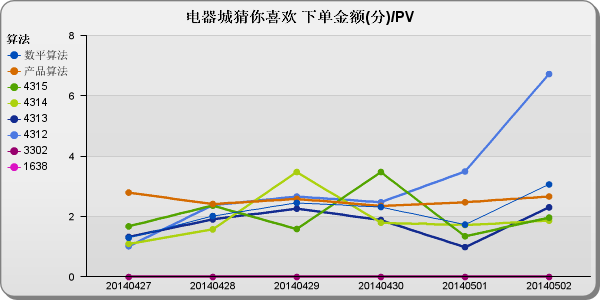
\includegraphics[width=0.8\textwidth]{fig/yixunexp/OAPI0427.png}
\caption{\label{fig:oapi0427} OAPI of online algorithms  from 0427 to 0502.}
\end{center}
\end{figure}
\end{frame}
\begin{frame}
  \frametitle{Online experiment results}
\begin{figure}
\begin{center}



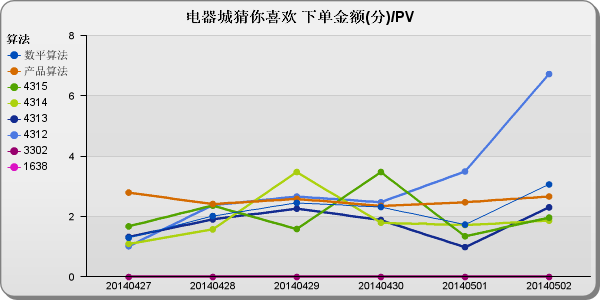
\includegraphics[width=0.8\textwidth]{fig/yixunexp/OAPI0427.png}
\caption{\label{fig:oapi0427} OAPI of online algorithms  from 0427 to 0502.}
\end{center}
\end{figure}
\end{frame}

\begin{frame}
  \frametitle{Online experiment results}
\begin{figure}
\begin{center}

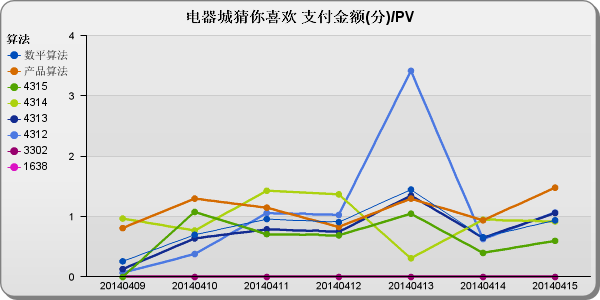
\includegraphics[width=0.8\textwidth]{fig/yixunexp/PAPI0415.png}
\caption{ PAPI of online algorithms  from 0409 to 0415.}
\end{center}
\end{figure}
\end{frame}
\end{section}

\begin{section}{Conclusion \& Future work}
  \begin{frame}
    \frametitle{Conclusion}
    \begin{itemize}
    \item Transfer learning for one-class CF.
      \begin{itemize}
      \item Matrix tri-factorization to share more data.
      \item Clustering-pattern transfer function.
      \end{itemize}
    \item Clustering based matrix factorization framework.
    \end{itemize}
  \end{frame}
  \begin{frame}
    \frametitle{Future work}
    \begin{itemize}
\item  Pair-wise Transfer Learning in CF.
\item  Online Transfer Learning in CF.
\item Transfer Learning in CF with multiple matrix.
\item Time Complexity Optimization in CF.
\end{itemize}
\end{frame}
\end{section}
\end{document}